\documentclass[11pt,letterpaper]{article}
\usepackage{naaclhlt2012}
\usepackage{times}
\usepackage{latexsym}
\usepackage{amsmath}
\usepackage{multirow}
\setlength\titlebox{6.5cm}    % Expanding the titlebox
\usepackage{url}
\usepackage{color}
\usepackage{colortbl}
\usepackage[vlined,figure]{algorithm2e}
\usepackage{graphicx} 

\DeclareMathOperator*{\argmax}{arg\,max}

\definecolor{red}{rgb}{1,0,0}
\definecolor{lightgray}{cmyk}{0,0,0,.08}

\newcommand{\mnote}[1]{\marginpar{%
  \vskip-\baselineskip
  \raggedright\footnotesize
  \itshape\hrule\smallskip\tiny{#1}\par\smallskip\hrule}}  

%\newcommand{\mtodo}[1]{}
\newcommand{\mtodo}[1]{\mnote{\textcolor{red}{#1}}}
\newcommand{\red}[1]{\textcolor{red}{#1}}
\newcommand{\todo}[1]{\textcolor{red}{TODO: #1}}
\newcommand{\todop}[2]{\noindent\textcolor{red}{TODO for #1:} #2\\}
\newcommand{\todopi}[2]{[\textcolor{red}{TODO for #1:} #2]}
\newcommand{\secref}[1]{Section~\ref{#1}}
\newcommand{\tabref}[1]{Table~\ref{#1}}
\newcommand{\figref}[1]{Figure~\ref{#1}}
\newcommand{\code}[1]{{\small \tt #1}}
\newcommand{\emq}[1]{\emph{``#1''}}
\newcommand{\paraheader}[1]{\vskip 0.05in \noindent\emph{#1}}
\newcommand{\skipheader}{\vskip 0.05in}

\newcommand{\bm}{\boldsymbol}
\def\bs#1{\boldsymbol{#1}}

\newenvironment{my_itemize}{
\begin{itemize}
  \setlength{\itemsep}{2pt}
  \setlength{\parskip}{2pt}
  \setlength{\parsep}{1pt}}{\end{itemize}
}


\title{Learning a Reordering Model Without Parallel Data}

%\author{}
% \author{Alex Klementiev \ \ \ \  Ann Irvine \ \ \ \ Chris Callison-Burch \ \ \ \ David Yarowsky \\
% Center for Language and Speech Processing \\ Johns Hopkins University}

%\author{Author 1\\
%	    XYZ Company\\
%	    111 Anywhere Street\\
%	    Mytown, NY 10000, USA\\
%	    {\tt author1@xyz.org}
%	  \And
%	Author 2\\
%  	ABC University\\
%  	900 Main Street\\
%  	Ourcity, PQ, Canada A1A 1T2\\
%  {\tt author2@abc.ca}}

\date{}

\begin{document}
\maketitle

\begin{abstract}
The parameters of statistical models of translation are typically estimated from large bilingual parallel corpora.  However, these resources are expensive to create and are unavailable for most language pairs.  In this work we consider estimating reordering probabilities for phrase-based machine translation from monolingual data alone.  We propose a novel algorithm and show it to be effective on three language pairs.
\end{abstract}

% ------------------------------------------------
\section{Introduction}

MT: (1) choose words (phrases) in the target language, (2) put them in the right order.  Both need parallel data, which is expensive.  In this work, we address the reordering problem using monolingual data alone, which is cheap and plentiful.  In this work, we assume that a phrase table is \emph{given} and only estimate the reordering features.  We study how the induced reordering model compares with its standard counterpart induced from parallel data.

% ------------------------------------------------
\section{Background} \label{sect:bckg}

\mtodo{Brief background on MT, reordering models.}

Statistical machine translation (SMT) was first formulated as a series of probabilistic models that learn word-to-word correspondences from sentence-aligned bilingual parallel corpora \cite{Brown:1993}.  \nocite{Brown1988}
%
Current methods, including {\em phrase-based} \cite{Och:2002,Koehn:2003} and {\em hierarchical} models \cite{Chiang:2005}, typically start by word-aligning a bilingual parallel corpus \cite{Och2003}.  They extract multi-word phrases that are consistent with the Viterbi word alignments, and use these phrases to build new translations.  Model parameters are estimated from large amounts of bitext.  One of those parameters is the reordering model

Each phrase pair $(e, f)$ has reordering parameters $p_o(\textnormal{orientation}|f,e)$ which indicate the distribution of its orientation with respect to the previously translated phrase. Orientations are {\it monotone, swap, discontinuous} \cite{tillman:2004:HLTNAACL,Kumar2004}, see \figref{fig:reorderfeats}. 

In this work, we keep the definition of the reordering features, but estimate them from monolingual data alone. 

\begin{figure}[t]
\begin{center}
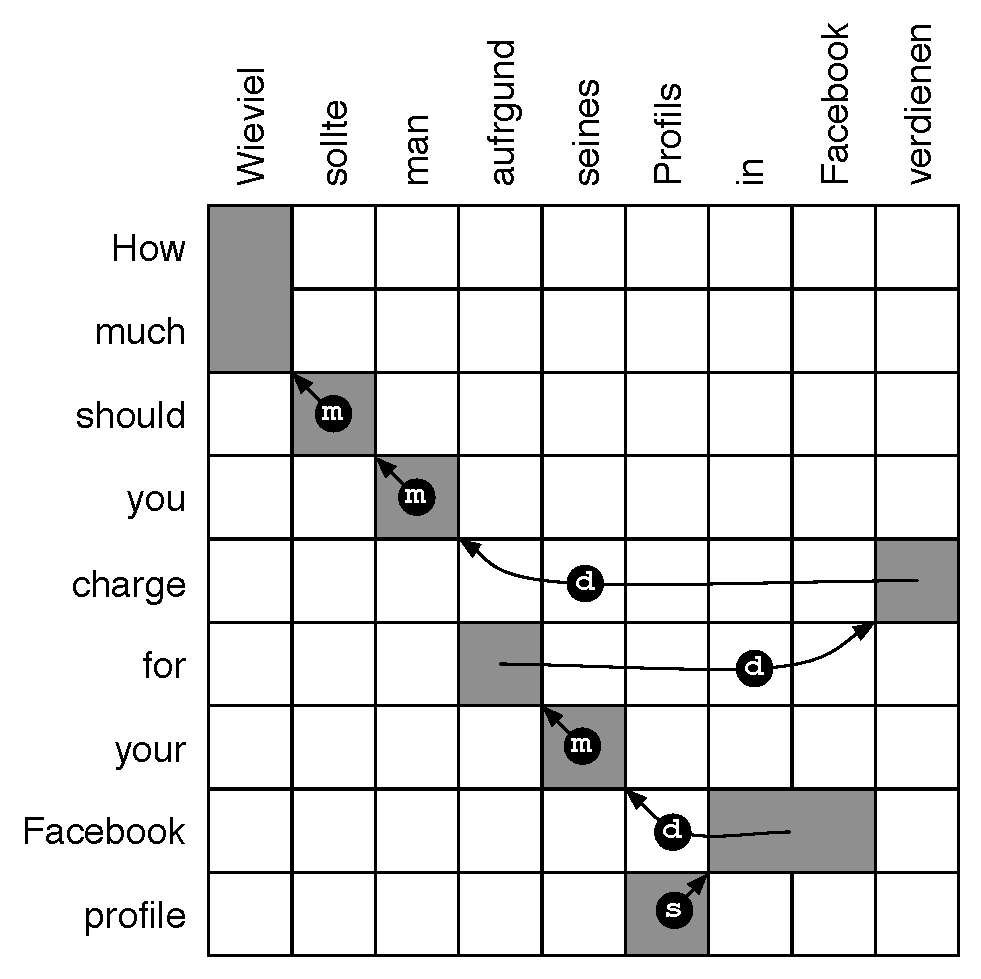
\includegraphics[width=0.8 \linewidth]{../figures/reorderfeats/reorderfeats.pdf}
\caption{The reordering probabilities from the phrase-based models are estimated from bilingual data by calculating how often in the parallel corpus a phrase pair $(f, e)$ is orientated with the preceding phrase pair in the 3 types of orientations (monotone, swapped, and discontinuous). }
\label{fig:reorderfeats} 
\end{center}
\end{figure}

% ------------------------------------------------
\section{Monolingual Reordering Estimation} \label{sect:order}

\SetAlFnt{\relsize{-1.5}}

\begin{algorithm}[t]

 \SetKwFunction{CollectOccurs}{CollectOccurs}
 \SetKwFunction{CollectPreceding}{CollectPreceding}
 \SetKwFunction{CollectFollowing}{CollectFollowing}
 \SetKwFunction{CollectDisc}{CollectDisc}
 \SetKwBlock{Body}{}{}
 \SetCommentSty{text}
 \SetFuncSty{text}

 \hrule \vskip 0.2cm

  \KwIn{Source and target phrases $f$ and $e$,\\
  \hskip 0.85cm Source and target monolingual corpora $\emph{C}_f$ and $\emph{C}_e$,\\
  \hskip 0.85cm Phrase table pairs $\emph{T} = \{(f^{(i)}, e^{(i)})\}_{i=1}^{N}$.}
  \KwOut{Orientation features ($p_m, p_s, p_d$).}
  
  \vskip 0.2cm \hrule \vskip 0.2cm

  $S_f \leftarrow$ sentences containing $f$ in $\emph{C}_f$\;
  $S_e \leftarrow$ sentences containing $e$ in $\emph{C}_e$\;
  
  $(B_f, -, -) \leftarrow \CollectOccurs(f, \cup_{i=1}^{N} f^{(i)}, S_f)$\;
  $(B_e, A_e, D_e) \leftarrow \CollectOccurs(e, \cup_{i=1}^{N} e^{(i)}, S_e)$\;
    
  $c_m = c_s = c_d = 0$\;
  
  \vskip 0.1cm 

  \ForEach{unique $f'$ in $B_f$} {
    \ForEach{translation $e'$ of $f'$ in $\emph{T}$} {

      $c_m = c_m + \#_{B_e}(e')$\; 
       $c_s = c_s + \#_{A_e}(e')$\; 
       $c_d = c_d + \#_{D_e}(e')$\; 
    }
  }
  
  $c \leftarrow c_m + c_s + c_d$;
    
  \Return{$({c_m \over c}, {c_s \over c}, {c_d \over c})$}

  \vskip 0.2cm \hrule \vskip 0.2cm

  \CollectOccurs{$r$, $R$, $S$} \Body{
   $B \leftarrow ()$; $A \leftarrow ()$; $D \leftarrow ()$\;

    \ForEach{sentence $s \in S$} {
      \ForEach{occurrence of phrase $r$ in $s$} {
        $B \leftarrow B$ $\cup$ \CollectPreceding{$r$, $R$}\;
        $A \leftarrow A$ $\cup$ \CollectFollowing{$r$, $R$}\;
        $D \leftarrow D$ $\cup$ \CollectDisc{$r$, $R$}\;
      }
    }
    
    \Return{($B$, $A$, $D$)}\;
  }
  
  \vskip 0.2cm \hrule \vskip 0.2cm

  \caption{Algorithm for estimating reordering probabilities from monolingual data.} \label{fig:algoreorder}
  \vskip -0.2in
\end{algorithm}


\begin{figure}[t]
%\vskip 0.1in
\begin{center}
%\vspace{-.85cm}
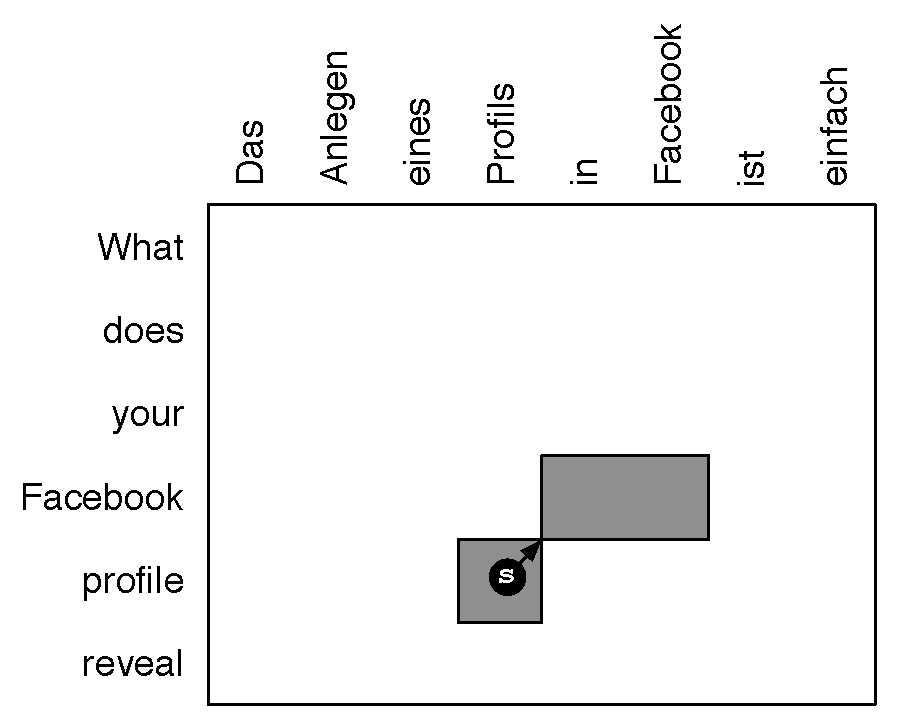
\includegraphics[width=0.8 \linewidth]{../figures/monoreord/monoreord.pdf}
%\vspace{-.25cm}
\caption{Collecting phrase orientation statistics for a English-German phrase pair (\emq{profile}, \emq{Profils}) from non-parallel sentences (the German sentence translates as  \emq{Creating a Facebook profile is easy}). %The longest preceding phrase \emq{Facebook} in source, has a phrase table translation \emq{in Facebook} appearing after the target phrase.
}
\label{fig:monoreord}
\end{center}
\vskip -0.2in
\end{figure}

We now introduce a novel algorithm for estimating $p_o(\textnormal{orientation}|f,e)$ from two monolingual corpora instead a bitext.

Figure \ref{fig:reorderfeats} illustrates how the phrase pair orientation statistics are estimated in the standard phrase-based SMT pipeline.  For a phrase pair like ($f =$ \emq{Profils}, $e =$ \emq{profile}), we count its orientation with the previously translated phrase pair ($f' =$ \emq{in Facebook}, $e' =$ \emq{Facebook}) across all translated sentence pairs in the bitext.  

In our setup we do not have translated sentence pairs.  Instead, we look for monolingual sentences in the source corpus which contain the source phrase that we are interested in, like $f =$ \emq{Profils}, and at least one other phrase that we have a translation for, like $f' =$ \emq{in Facebook}.  We then look for all target language sentences in the target monolingual corpus that contain the translation of $f$ (here $e =$ \emq{profile}) and any translation of $f'$.  \figref{fig:monoreord} illustrates that it is possible to find evidence for $p_o(\textnormal{swapped}| \it{ Profils},\it{ profile})$, even from the non-parallel, non-translated sentences drawn from two independent monolingual corpora.  By looking for foreign sentences containing pairs of adjacent foreign phrases $(f, f')$ and English sentences containing their corresponding translations $(e, e')$, we are able to increment orientation counts for $(f, e)$ by looking at whether $e$ and $e'$ are adjacent, swapped, or discontinuous, much in the same way as in Fig.~\ref{fig:reorderfeats}.


%In the phrase-based SMT pipeline, phrase pair orientation statistics are collected using word alignments.  We keep a similar reordering model formulation but infer its parameters from monolingual data instead.  The orientation information for a phrase pair ($f$, $e$) is collected from source and target sentences containing ($f$, $e$) as well as other phrase pairs.  Suppose one such sentence pair contains another pair of phrases ($f'$, $e'$), and that $f'$ is immediately adjacent to $f$.  The idea is to check whether $e'$ stays in the same order with $e$, swaps, or becomes discontinuous in the target sentence. Consider the simple example in \figref{fig:monoreord}: the phrase pair is ($f =$ \emq{profile}, $e =$ \emq{Profils}), and a given pair of non-parallel sentences also contains a phrase table entry ($f' =$ \emq{Facebook}, $e' =$ \emq{in Facebook}).  In this example, the phrase $f'$ preceding $f$ in the source sentence swaps order with $e$ in the target.  When we collect these counts over large monolingual corpora, we expect the swap, monotone, and discontinuous counts to provide good estimates for the orientation features (\figref{fig:algoreorder}).
%Note that multiple phrases may immediately precede $f$ and appear in the phrase table; however, we only use the longest of them to collect reordering counts.  

Contextual phrases for a given phrase \code{r} are only collected (in \code{CollectPreceding}, \code{CollectFollowing}, and \code{CollectDisc} on figure \figref{fig:algoreorder}) if they also appear in phrase table \code{R}.  Note that shorter and more frequent phrases (e.g. punctuation) are more likely to appear in multiple orientations with a given phrase, and therefore provide poor evidence of re-ordering.  Therefore, when collecting contextual phrases for reordering feature estimation, we:

\begin{itemize}
  \item Keep only the longest contextual phrases (which also appear in the phrase table).
  \item Prune the set of phrases so that we only keep a small set of least frequent contextual phrases (this has the effect of dropping many function words and punctuation marks and and relying more heavily on multi-word content phrases to estimate the reordering).\footnote{The pruning step has an additional benefit of minimizing the memory needed for orientation feature estimations.}
  \item Do not look too far away from a given phrase when collecting discontiguous phrases in \code{CollectDisc}.
\end{itemize}

We empirically investigate the effect of all of these choices in \secref{sect:eval}.

% ------------------------------------------------
\section{Empirical Evaluation} \label{sect:eval}

In this work, we assume that a phrase table induced from parallel data is given but estimate phrase pair reordering features from monolingual data.  We evaluate the induced reordering features in two ways: (a) compare the induced reordering preferences with those induced from bitext in the standard phrase-based MT pipeline using a metric we define below, and (b) use them in place of the bitext estimated reordering model in a complete SMT pipeline.

\paraheader{Data.} We estimate our reordering features from (a subset of) the Gigaword corpus for English, Spanish, German, and the wikipedia data for Urdu.

\paraheader{Evaluation metrics.} We evaluate the induced reordering both in the complete system and using the following metric. \todo{Define}.  Intuitively, it measures how well the monolingual reordering features agree with their bilingually estimated counterparts in their ordering preferences for a given phrase.

% ------------------------------------------------
%\section*{Acknowledgments}

%Do not number the acknowledgment section.

\bibliographystyle{naaclhlt2012}
\bibliography{reorder}

\end{document}
